
\begin{correction} \;
C'est une suite de type $u_{n+1}=f(u_n)$, on donne les id\'ees de l'\'etude. Ainsi la r\'edaction dans une copie doit \^{e}tre beaucoup plus d\'etaill\'ee qu'ici.
\begin{enumerate}
 \item \'Etude de la fonction $f$ associ\'ee: $x\mapsto \ddp\frac{(1+x)^2}{4}$\\
\noindent La fonction $f$ est d\'efinie, continue et d\'erivable sur $\R$ et 
$$\forall x\in\R,\ f^{\prime}(x)=\ddp\frac{1+x}{2}.$$
On obtient ainsi le tableau de variation suivant:
\begin{center}
\begin{tikzpicture}
 \tkzTabInit{ $x$          /1,%
       $f'(x)$      /1,%
       $f$       /2}%
     { $-\infty$, $-1$ ,$+\infty$ }%
  \tkzTabLine {,-,0,+,}%
  \tkzTabVar{
       +/ $+\infty$        /,
        -/$0$           /,%
       +/$+\infty$           /,
                      }
 \tkzTabVal[draw]{2}{3}{0.3}{$0$}{$\frac{1}{4}$}
  \tkzTabVal[draw]{2}{3}{0.6}{$1$}{$1$}
\end{tikzpicture}
\end{center}
\item Calcul des limites \'eventuelles:\\
\noindent La fonction $f$ est continue sur $\R$, ainsi, si la suite $\suiteu$ converge, elle ne peut converger que vers $l$ v\'erifiant 
$$l=f(l)\Leftrightarrow l=1.$$
Ainsi, 1 est la seule limite \'eventuelle de la suite.
\item La suite est bien d\'efinie et elle appartient \`{a} $I$ intervalle stable par $f$:\\
\noindent On remarque que $\lbrack 0,1\rbrack$ est un intervalle stable par $f$ et que $u_0=0\in\lbrack 0,1\rbrack$. Un raisonnement par r\'ecurrence permet alors de v\'erifier que la suite est bien d\'efinie et que:
$$\forall n\in\N,\quad u_n\in\lbrack 0,1\rbrack.$$
\noindent 
\item \'Etude de la monotonie de la suite:\\
La fonction $f$ est croissante sur $\lbrack 0,1\rbrack$ et la suite $\suiteu$ est bien \`a valeurs dans $\lbrack 0,1\rbrack$, ainsi, la suite $\suiteu$ est monotone. Il suffit alors de comparer $u_1$ et $u_0$ et on obtient
$$u_1=\ddp\frac{1}{4}>u_0.$$
Ainsi, un raisonnement par r\'ecurrence permet de montrer que la suite $\suiteu$ est croissante (voir les exemples du cours, le raisonnement par r\'ecurrence est obligatoire).
\noindent 
\item \'Etude de la convergence de la suite:\\
\noindent La suite $\suiteu$ est ainsi croissante et major\'ee par 1, elle converge donc vers une limite finie $l\in\R$ d'apr\`es le th\'eor\`eme sur les suites monotones. De plus, comme la seule limite \'eventuelle est 1, on sait que la suite $\suiteu$ converge vers 1.
\end{enumerate}
\end{correction}